\section{Filtro pasaaltos}

\subsection{Análisis teórico}

\subsubsection{Modelos ideales}

Al igual que en el análisis del filtro pasabajos se supondrá que tanto el generador como los componentes a medir son ideales, es decir, se desprecia toda variación de sus características eléctricas

\begin{figure}[H]
    \centering
    \begin{circuitikz}[american voltages]
            \tikzstyle{every node}=[font=\footnotesize]	
            \draw
            (0,-1) to[american voltage source, l=$v\left(t\right)$, invert] ++(0,2) -- ++(0.5,0)
            to[C, l=$C$, v=$v_c$, i=$i\left(t\right)$] ++(2,0) -- ++(0.5,0) node[]{}
            to[R, l=$R$, v=$v_r$] ++(0,-2)
            to[short, -*] ++ (-1.5,0) node[ground, scale=0.6]{} to[short] ++(-1.5,0);
    \end{circuitikz}
    \caption{Circuito te\'orico RC}
    \end{figure}

De este circuito se deriva la función transferencia que lo caracteriza, expresada en la ecuación~\ref{eq:pasaaltos_transferencia}

\begin{equation}\label{eq:pasaaltos_transferencia}
    H(s) = \frac{V_R}{V_i} = \frac{R}{\frac{R \cdot C \cdot s +1}{C \cdot s}}
    = \frac{s \cdot R \cdot C}{s \cdot R \cdot C + 1} 
\end{equation}

Si se asume que el sistema es LTI, causal y BIBO-estable se puede obtener la respuesta en frecuencia del mismo haciendo el reemplazo $s = j\omega$, resultando en: 

\begin{equation}\label{eq:pasaaltos_rta_frecuencia}
    H(f) = \frac{2\pi \cdot f \cdot R \cdot C}{2\pi \cdot f \cdot R \cdot C + 1}
\end{equation}

Como podemos observar en la ecuación~\ref{eq:pasaaltos_rta_frecuencia} el sistema presenta un cero en $f_0 = 0$ y un polo simple en $f_1 = \frac{1}{R \cdot C}$.

\subsubsection{Modelo equivalente del capacitor}

En el apartado anterior se hizo mención de la idealidad de los componentes a la hora de hacer un análisis sobre el circuito.
 Para obtener una aproximación más cercana al comportamiento real del mismo, incorporamos el modelo paralelo del capacitor a las ecuaciones.

 %%INSERTAR CIRCUITO CON MODELO PARALELO DEL CAPACITOR
 \begin{equation*}
    AGREGAR CIRCUITO CON MODELO PARALELO DE CAP (tikz)
 \end{equation*}


 De este circuito se puede obtener una nueva expresión de función transferencia, como se observa en la figura~\ref{eq:pasaaltos_transferencia_modcap}.

 \begin{equation}\label{eq:pasaaltos_transferencia_modcap}
    H(s) = \frac{s \cdot C \cdot R \cdot R_c + R}{s \cdot C \cdot R \cdot R_c + R + R_c}
\end{equation}

De la anterior ecuación se puede deducir que cambiarán los valores de frecuencia del polo y del cero calculados anteriormente, en condiciones ideales.

\subsection{Mediciones y resultados}

En esta sección se volcarán los datos obtenidos de las mediciones en laboratorio del filtro. Cabe destacar que los componentes empleados para tal fin son idénticos a los utilizados en el análisis del pasabajos.
De igual manera, se usó las puntas del osciloscopio en modo x10 (previa calibración de las mismas) de forma tal de minimizar el impacto de estas sobre el circuito.

%\subsubsection*{Frecuencia de corte real}
%
%En este apartado buscaremos la frecuencia real de corte del circuito. Esto se puede llevar a cabo inyectando una señal sinusoidal en la entrada del filtro, de frecuencia ajustable. 
%Con ayuda de un osciloscopio para observar la diferencia de fase entre entrada y salida, se realiza un barrido en frecuencia hasta alcanzar un valor de fase de $45°$.
%
%\begin{table}[H]
%	\begin{center}
%		\begin{tabular}{c c c c c}
%		$C$ & $Re(Y_C)$ & $Im(Y_C)$ & $Re(Z_R)$ & $Im(Z_R)$ \\
%		\hline
%		$1,46nF$ & $\frac{1}{55,5k \Omega}$ & $\frac{j}{5,446k \Omega}$ & $5,46k \Omega$ & $-j2,85 \Omega$
%		\end{tabular}
%		
%		\caption{Mediciones con analizador de impedancias}
%	\end{center}
%\end{table}

En un principio, se excitó a la entrada con una señal sinusoidal de amplitud $20V_{pp}$ barriendo la frecuencia de la misma. La amplitud elegida es la máxima entregable por el generador de señales.
 Cuanto mayor sea la amplitud de excitación se apreciará menos el nivel de ruido electromagnético, colaborando con la medición. En un principio, se barrió en un espectro de frecuencias desde $10Hz$ hasta 1$Mhz$.
 Se hizo énfasis en las zonas críticas del diagrama para poder obtener una curva representativa. En la tabla~\ref{table:pasaaltos_rta_frec_table} se reflejan los valores medidos de tensión de entrada y salida, y la diferencia de fase entre estos.

 \begin{table}[H]
 \centering
	\begin{tabular}{c c c c c}
		$\bm{f}$ & $\bm{v_g}$ & $\bm{v_R}$ & $\bm{\frac{V_R}{V_g}db}$ & 
		$\bm{\theta_{\Delta t}}$ \\ \hline
		\csvreader[head to column names, late after line=\\]{../Mediciones/Excel/pasaaltos_rta_frec.csv}{}{\frecuencia & \vin & \vout & \phase}
		\hline
	\end{tabular}
	\label{table:pasaaltos_rta_frec_table}
	\caption{Mediciones del m\'odulo de la respuesta en frecuencia}
\end{table}

 Cabe aclarar que para la medición de fase entre señales emplemos el método $\Delta t$, dado que consideramos que introduce menos error al proceso debido a la menor intervención humana en interpretación, respecto al modo \textsc{XY}.

 En la figura~\ref{pasaaltos_bode} se puede observar la superposición del BODE teórico calculado y el mismo diagrama resultante de la medición sobre el circuito.

 \begin{figure}[H]
    \centering
    \includegraphics[width = 0.9\textwidth]{../Desarrollo/pasaaltos_bode_amp.png}
    \caption{Diagrama BODE de amplitud}
    \label{fig:pasaaltos_bode_amp}
 \end{figure}

 \begin{figure}[H]
    \centering
    \includegraphics[width = 0.9\textwidth]{../Desarrollo/pasaaltos_bode_pha.png}
    \caption{Diagrama BODE de fase}
    \label{fig:pasaaltos_bode_phase}
 \end{figure}

 En ambos casos podemos observar la simmilitud entre las curvas teóricas y las medidas. Las diferencias están en los intervalos de toma de datos de la medición, dado que la cantidad de puntos medidos es considerablemente menor a la cantidad de puntos calculados.
  Por otro lado, también pueden existir diferencias dadas las tolerancias de los componentes, la temperatura a la que funciona el circuito, resistencias en los cables y conexiones, ruido electromagnético, etc. 
 Además también podemos incluir la perturbación que subyace a la conexión las puntas del osciloscopio, dado que se agrega una impedancia capacitiva en paralelo que afecta las características del filtro (como por ejemplo la frecuencia de corte).

 \subsubsection*{Respuesta a señal triangular}

 Se excitó al circuito con una señal del tipo triangular, con un valor de tensión pico a pico $V_{pp}=20V$ (el máximo permitido por el generador). 
 En particular, se midió el circuito en tres casos de frecuencia de entrada ($f_0=2kHz, f_1=20kHz, f_2=100kHz$).


El caso de la frecuencia baja ($f_0=2kHz$) está reflejado en la figura~\ref{fig:pasaaltos_triangular_baja}. En esta imagen podemos apreciar como la salida se asemeja a una señal cuadrada.
 Luego, el sistema se comporta como un integrador. Los vértices de la salida cuadrada se ven distorsionados presuntamente por las curvas características de carga y descarga del capacitor asociado al filtro.
 Además la atenuación en la salida es considerable, de acuerdo al análisis teórico realizado con anterioridad.

 \begin{figure}[H]
    \centering
    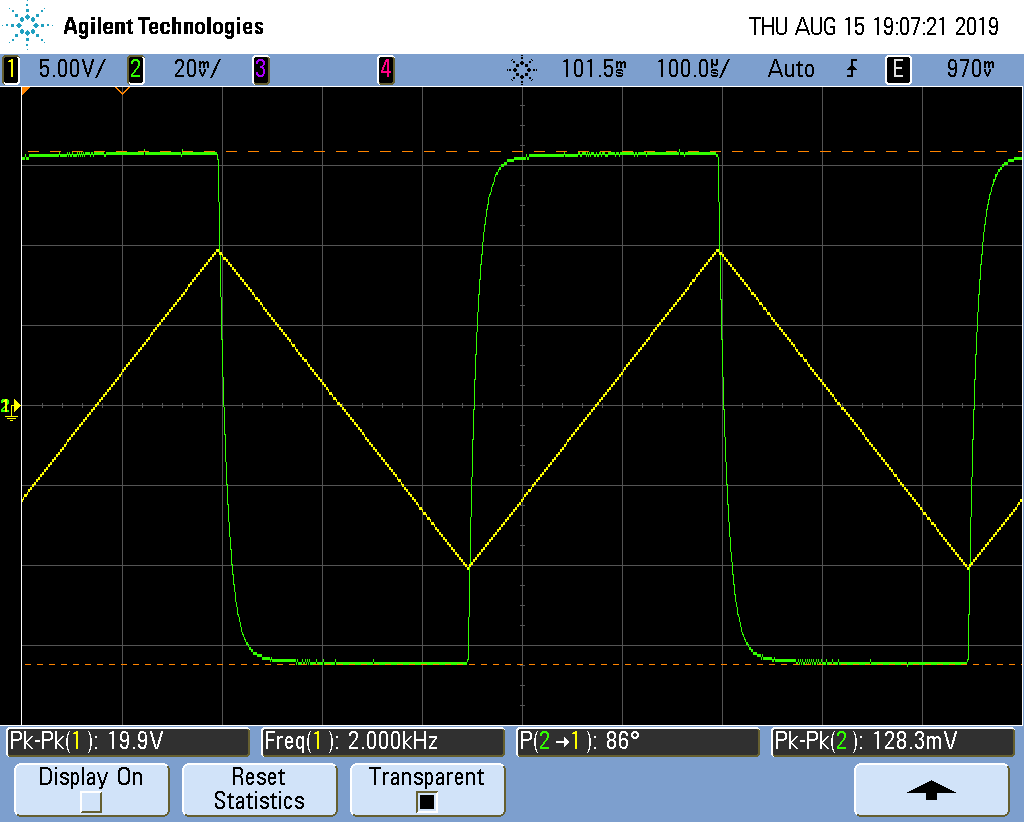
\includegraphics[width = 0.9\textwidth]{../Desarrollo/pasaaltos_triangular_2k.png}
    \caption{Respuesta a señal triangular de frecuencia $f=2kHz$}
    \label{fig:pasaaltos_triangular_baja}
 \end{figure}
 
Si ahora se aumenta la frecuencia de la señal en una década se puede observar como la señal de salida tiende a ser triangular, pero con los lados curvos. Esto es nuevamente debido a la presencia del capacitor en el circuito, que se carga y descarga, deformando así la señal de salida.

 \begin{figure}[H]
    \centering
    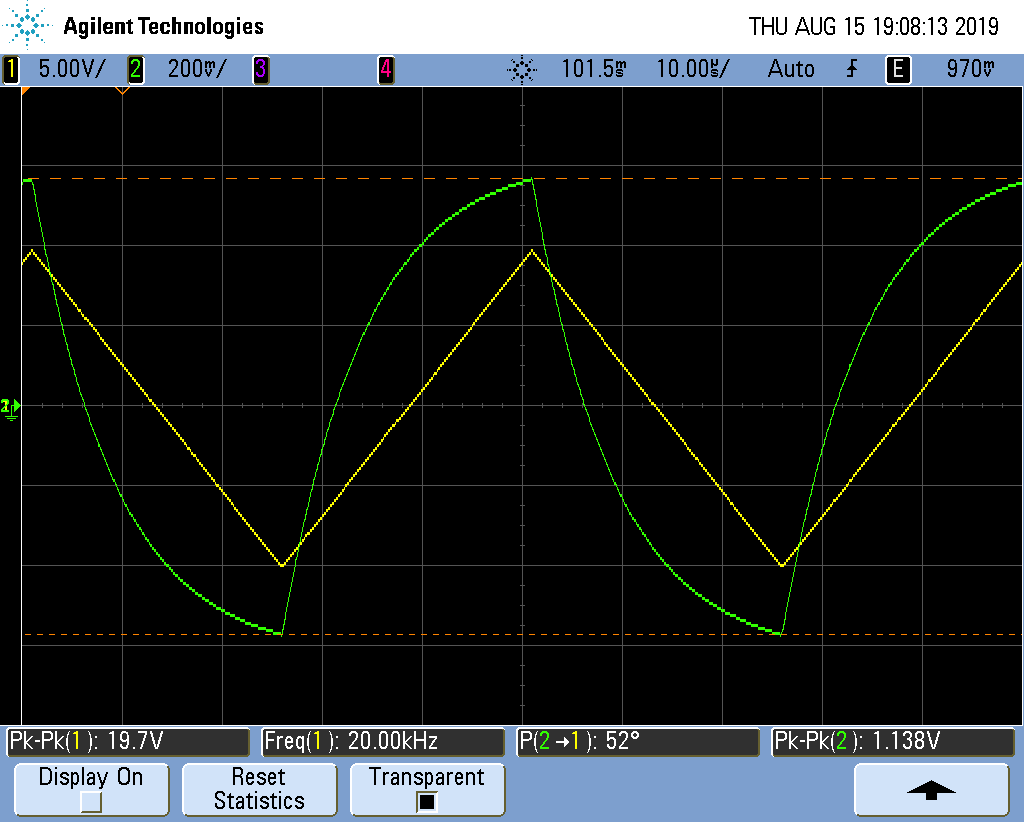
\includegraphics[width = 0.9\textwidth]{../Desarrollo/pasaaltos_triangular_20k.png}
    \caption{Respuesta a señal triangular de frecuencia $f=20kHz$}
    \label{fig:pasaaltos_triangular_media}
 \end{figure}

Por último, si forzamos la frecuencia a $f=100Hz$ se observa que la señal se asemeja aún mas a la función triangular de entrada. En este caso la curva en los lados es de un radio mayor. Además se aprecia que la atenuación de la señal sigue siendo considerable, pero mucho menor a los casos anteriores.

 \begin{figure}[H]
    \centering
    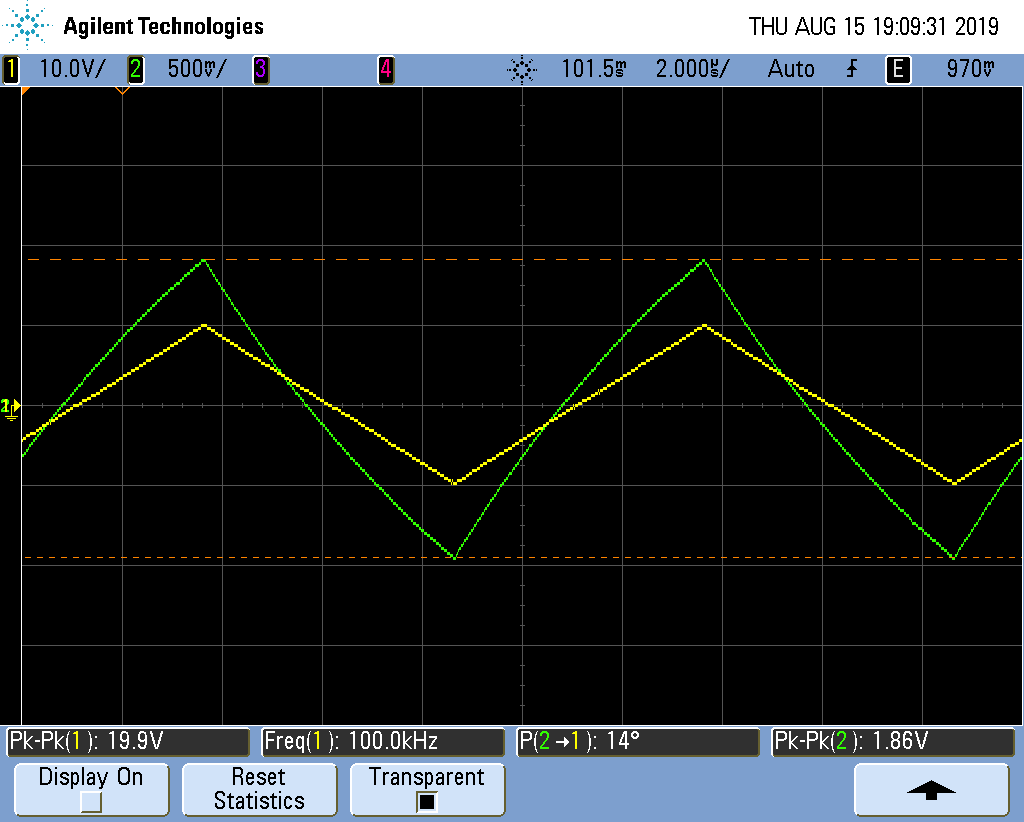
\includegraphics[width = 0.9\textwidth]{../Desarrollo/pasaaltos_triangular_100k.png}
    \caption{Respuesta a señal triangular de frecuencia $f=100kHz$}
    \label{fig:pasaaltos_triangular_alta}
 \end{figure}

 En resumen, podemos apreciar como al aumentar la frecuencia la señal tiende copiar la forma de la entrada. Esto es lógico debido a que se está analizando un filtro pasaaltos.
  Además, como se observa en la ecuacion~\ref{eq:pasaaltos_rta_frecuencia} la respuesta en frecuencia es un cociente de polinomios de grado 1, cuyos coeficientes principales son idénticos.
  Luego, para valores de frecuencia altos comparables con la frecuencia de corte del filtro todo el cociente tiende a la unidad.
